\chapter{Database Design}

\section[User Roles]{User and User Roles}

This is crucial to maintain database security via RBAC (Role-Based Access Control).

\begin{figure}[h]
	\centerline
	{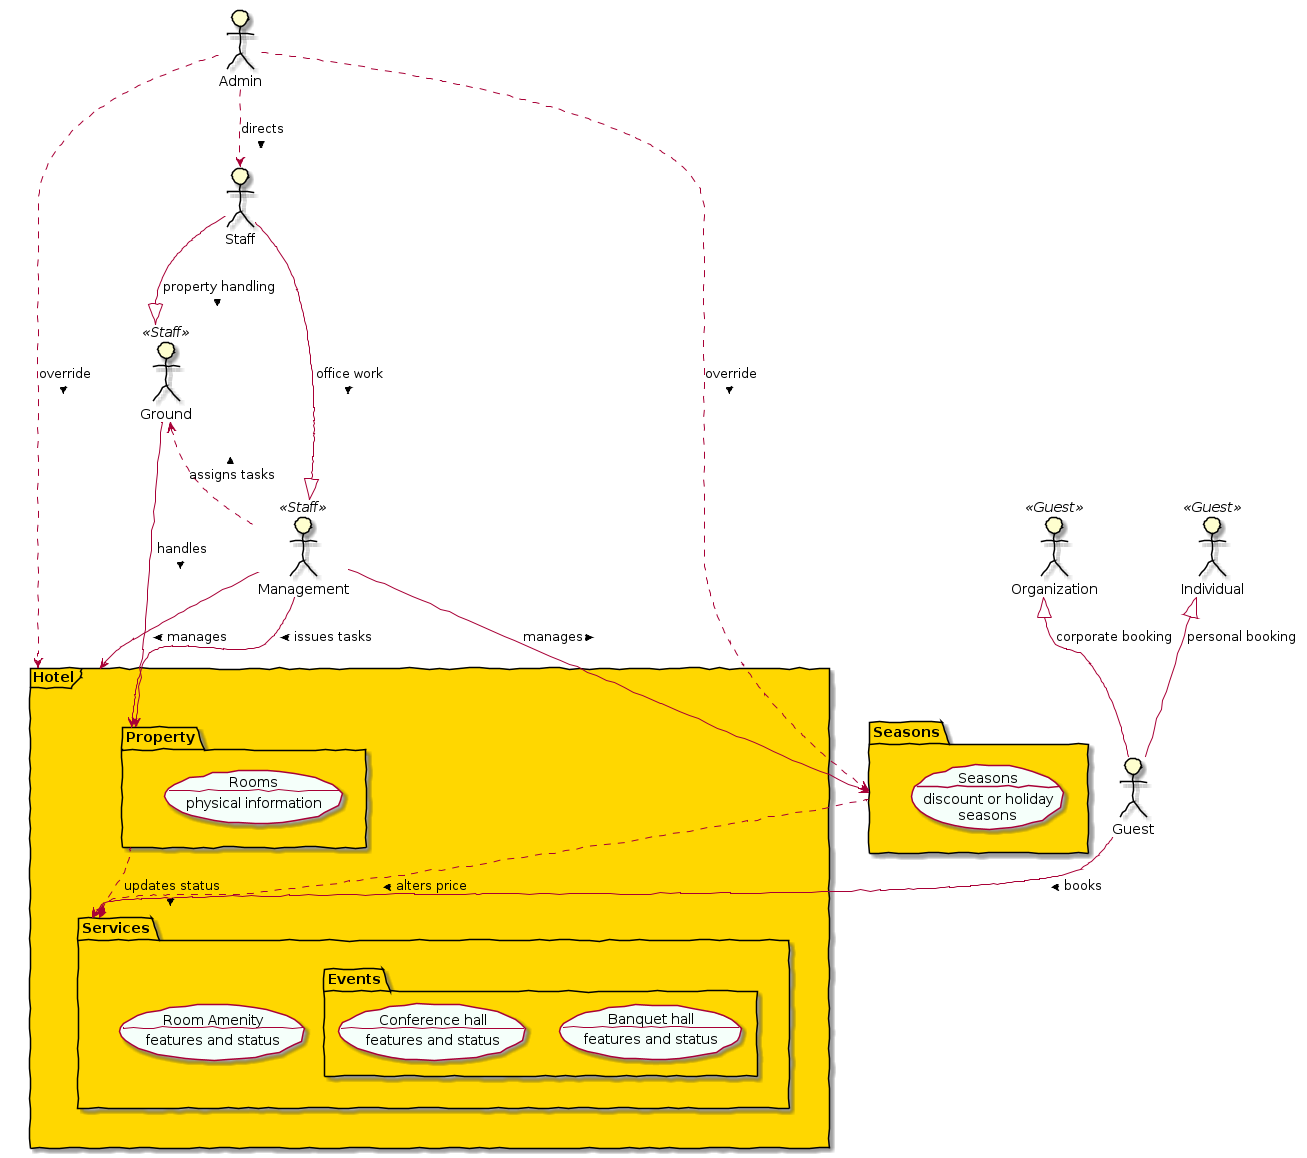
\includegraphics[width=15cm]{fig/HotelUseCase}}
	%{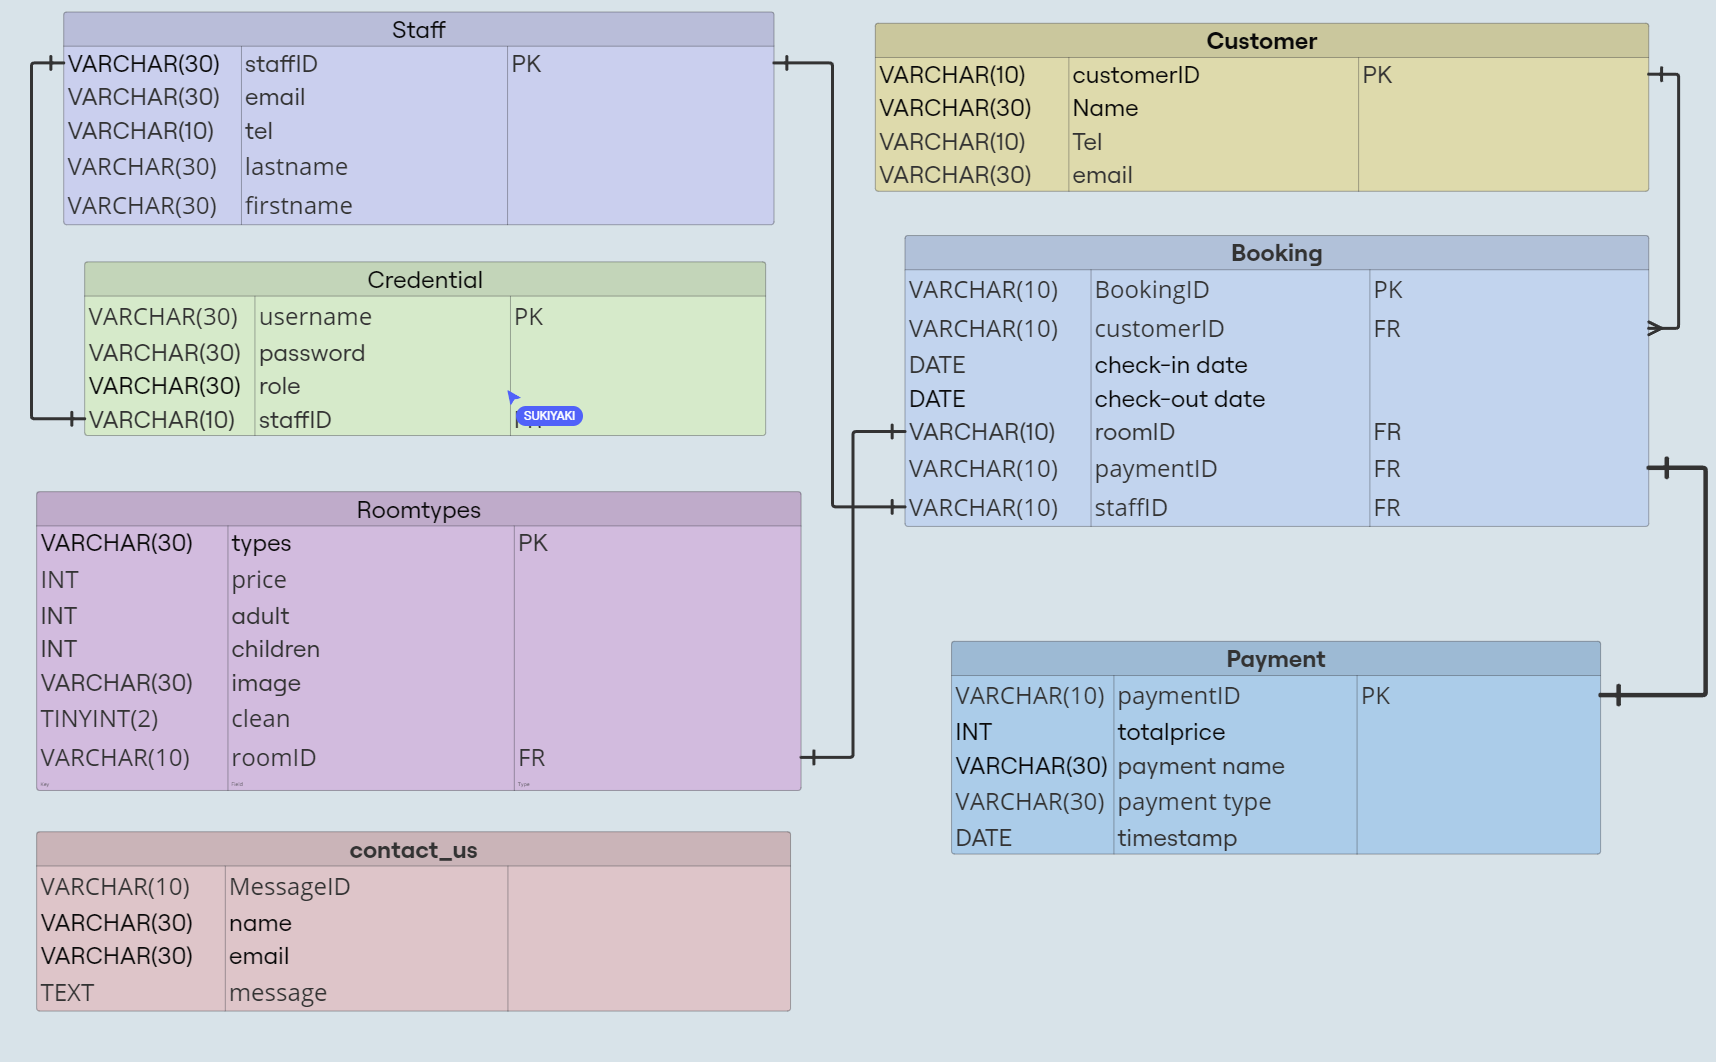
\includegraphics[]{fig/ERD_v1}}
	\caption{Use case diagram to represent actors and entities}
\end{figure}

As from the premise in chapter 1, we have three major user types of our applications: \textbf{admin}, \textbf{staff} and \textbf{guest}. \textbf{Staff} is further separated into \textbf{management} and \textbf{ground} staff. Likewise, \textbf{guest} is also separated such that they can guest entity can represent \textbf{individual} or an \textbf{organizations}. This comes handy since guests reserving these properties would like to taxes on their expenses in various fashions. Therefore, we have following major user roles:

\begin{enumerate}
	\item Admin
	\item Management \texttt{<staff>}
	\item Ground \texttt{<staff>}
	\item Individual \texttt{<guest>}
	\item Organization \texttt{<guest>}
\end{enumerate}

\subsection{User Roles Design for RBAC}

For reference, we use \texttt{A} for Add, \texttt{V} for View, \texttt{E} for Edit, and \texttt{D} for Delete to represent user roles.

\begin{table}[H]
	\centering
	\begin{tabular}{clllll}
		\hline
		Relation & Admin (DBA) & Management \texttt{<staff>} & Ground \texttt{<staff>} & Guest (both) \\ \hline
		\texttt{Hotel-Basic-Info} & \texttt{V, A, E, D} & \texttt{V} & \texttt{V} & \texttt{V}  \\
		\texttt{Facility-Info} & \texttt{V, A, E, D} & \texttt{V, A, E} & \texttt{V} & \texttt{V}  \\
		\texttt{Property-Info} & \texttt{V, A, E, D} & \texttt{V, A, E} & \texttt{V} & \texttt{V}  \\
		\texttt{Service-Info} & \texttt{V, A, E, D} & \texttt{V, A, E} & \texttt{-} & \texttt{V}  \\
		\texttt{Staff-Info} & \texttt{V, A, E, D} & \texttt{V (self)} & \texttt{V (self)} & \texttt{-}  \\
		\texttt{Mgmt-Staff-Info} & \texttt{V, A, E, D} & \texttt{V} & \texttt{-} & \texttt{-}  \\
		\texttt{Contact-Ticket} & \texttt{V, A, E, D} & \texttt{V, E} & \texttt{-} & \texttt{V, A (self)}  \\
		\texttt{Ground-Staff-Info} & \texttt{V, A, E, D} & \texttt{V} & \texttt{V (self)} & \texttt{-}  \\
		\texttt{Ground-Task-Info} & \texttt{V, A, E, D} & \texttt{V, A, E} & \texttt{V (self)} & \texttt{-}  \\
		\texttt{Ground-Task-Ticket} & \texttt{V, A, E, D} & \texttt{V, A, E, D} & \texttt{V, E (self)} & \texttt{-}  \\
		\texttt{Guest-Info} & \texttt{V, A, E, D} & \texttt{V} & \texttt{-} & \texttt{V, A, E, D (self)}  \\
		\texttt{Seasons-Discount-Info} & \texttt{V, A, E, D} & \texttt{V} & \texttt{-} & \texttt{V}  \\
		\texttt{Reservations} & \texttt{V, A, E, D} & \texttt{V, A, E, D} & \texttt{-} & \texttt{V, A (self)}  \\
		\texttt{Invoice} & \texttt{V, A, E, D} & \texttt{V, A, E} & \texttt{-} & \texttt{V, A (self)}  \\
		\hline
	\end{tabular}
	\caption{Major user roles}
\end{table}

For abstraction, both individual and guests representing organization are hold under same entity. This can be customized later based on customer feedback. Also, we would like to merge upper management to Admin access and use Management \texttt{<staff>} entity for field level management. This is for not allowing all levels of managerial positions have Admin level access. However, in small hotels upper management usually has data access up to admin level in absence of owner.

\subsection{Relation Design}

\section[ER Model]{ER Model Diagram}

ER model represents business needs to remember in order to perform business operations. \cite{Bagui2022} Among different diagramming convention techniques used to represent ER model of the database, we selected UML class diagram. We prefer this over originally accepted Chen's notation considering its extensive ability to describe multiplicity between the relationships. \cite{broy_entity-relationship_2002}

The final version of ER model is presented in Figure 3.3. We have separated areas of concerns such as staff management, business management and property management into different packages. This helps development teams to split tasks on specific domains and develop each packages individually.

\begin{figure}[h]
	\centerline
	{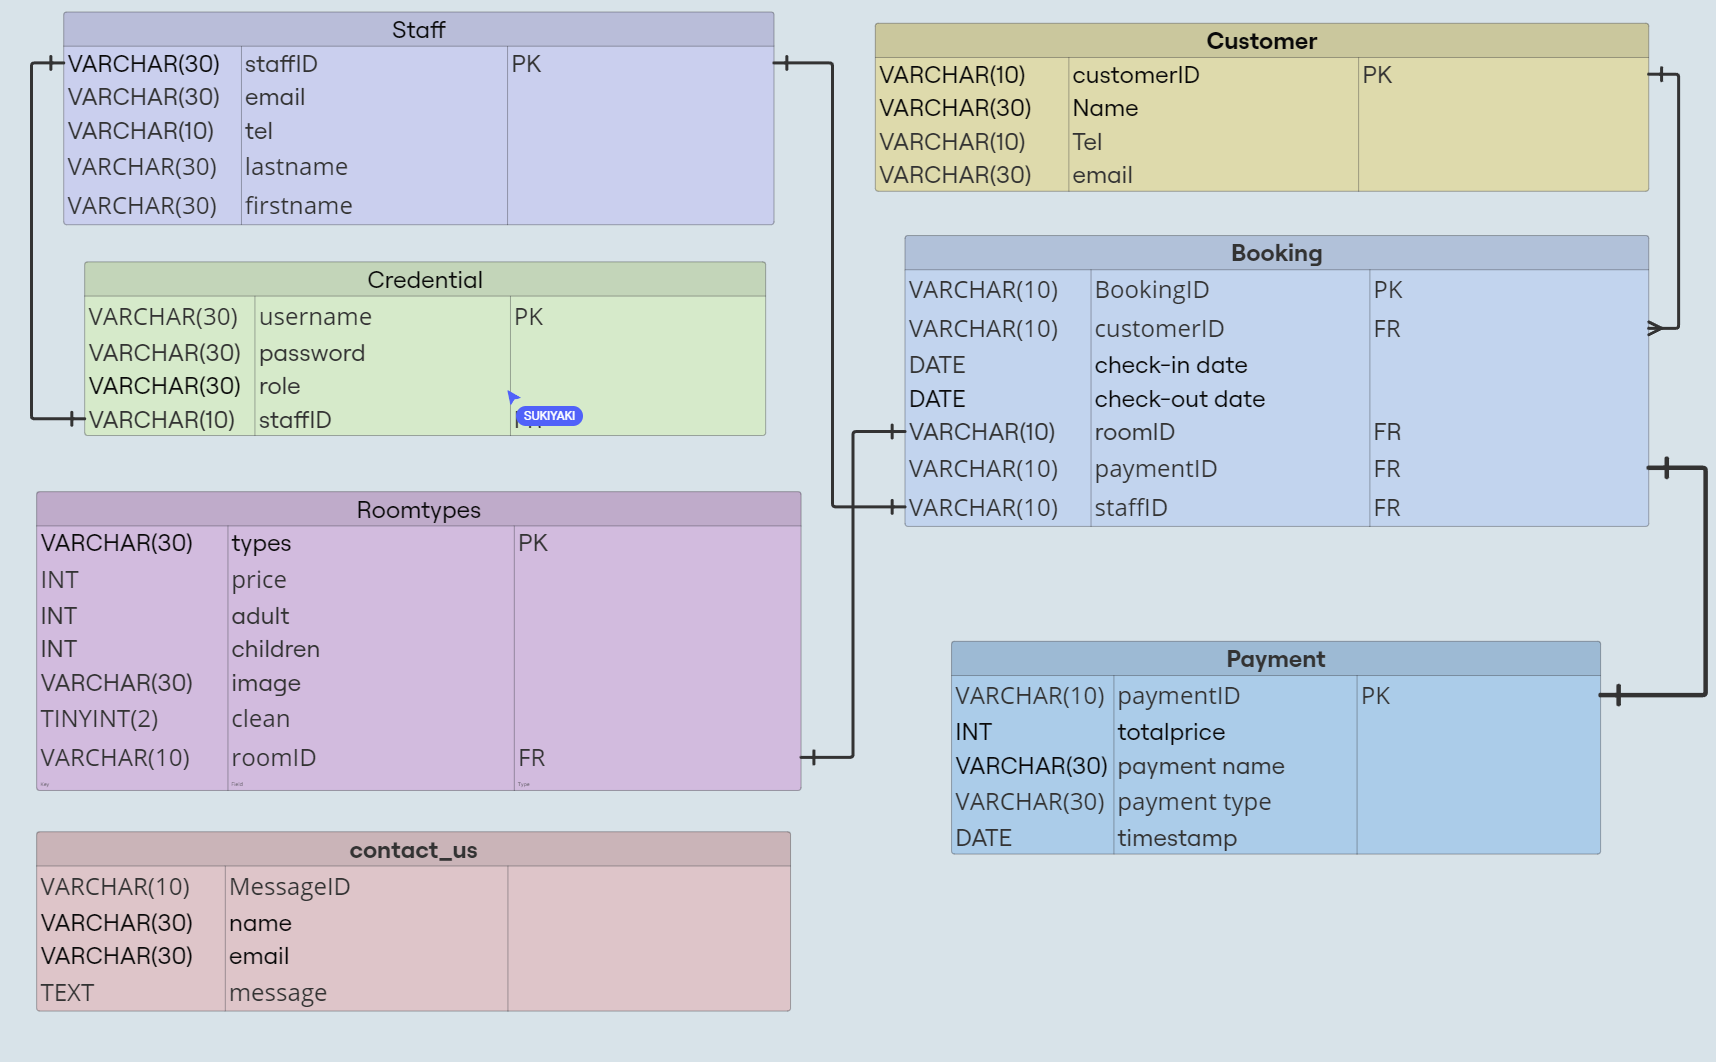
\includegraphics[width=15cm]{fig/ERD_v1}}
	%{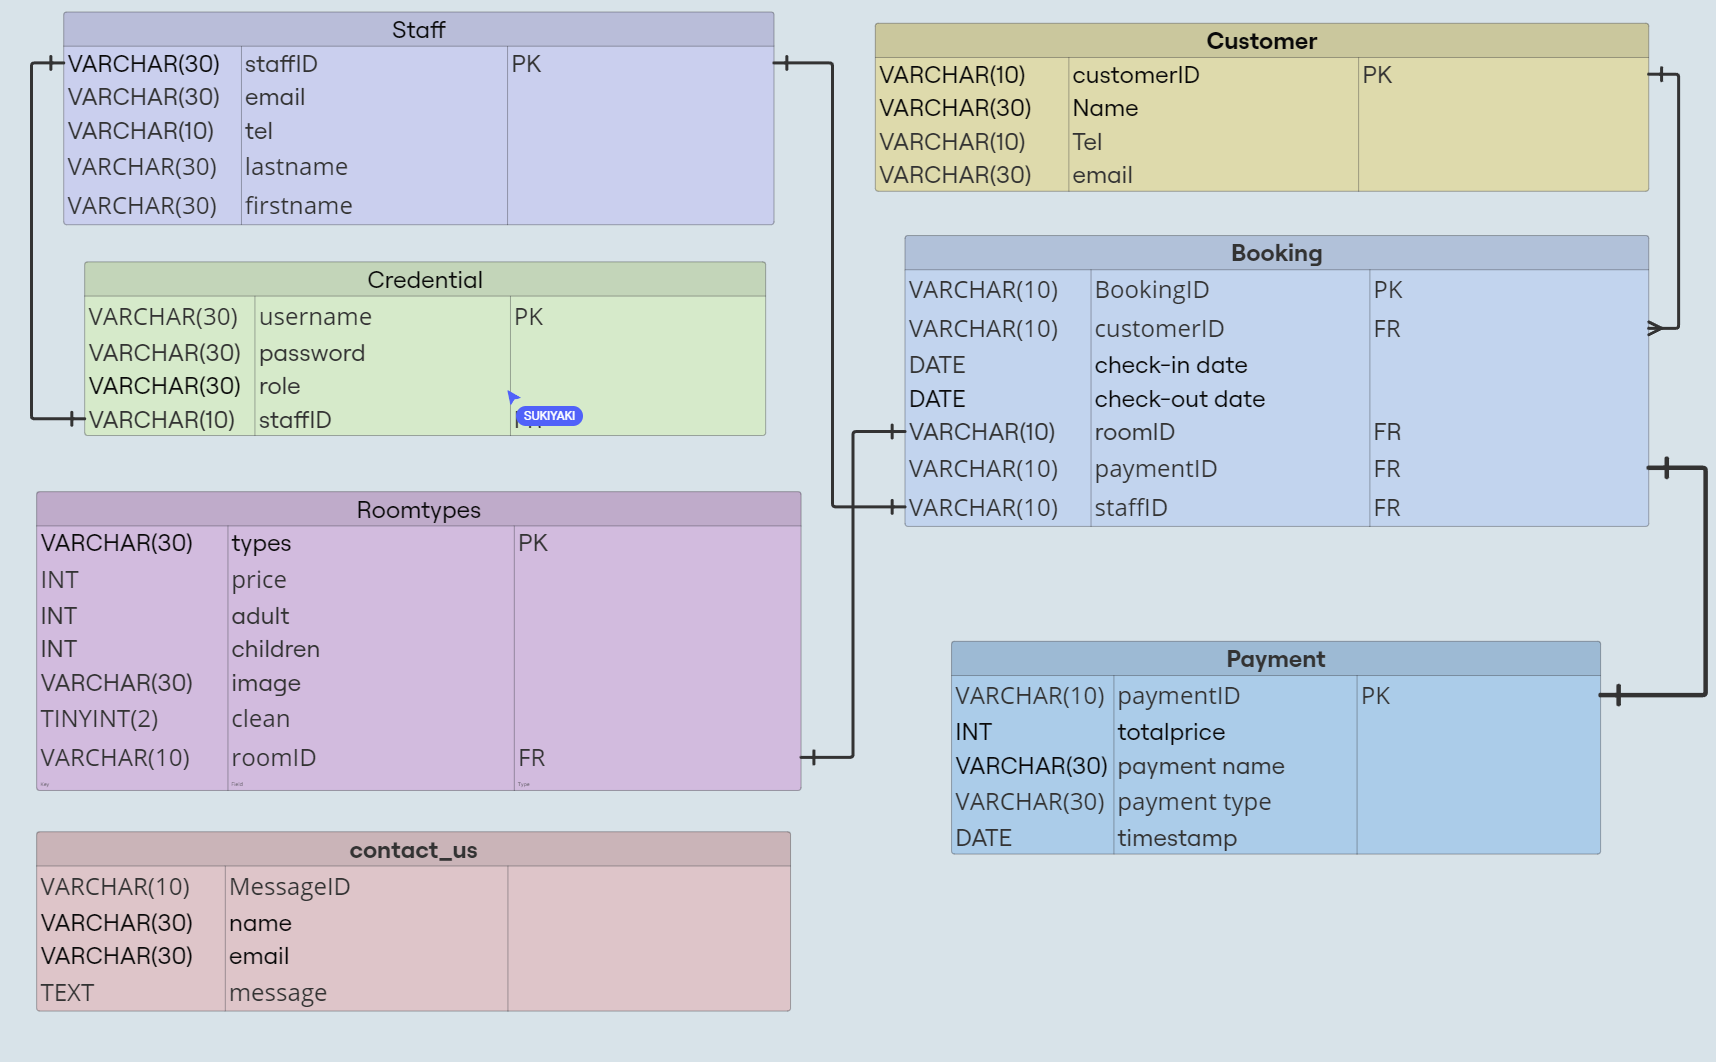
\includegraphics[]{fig/ERD_v1}}
	\caption{Initial draft for ER model diagram}
\end{figure} 

\begin{figure}[h]
	\centerline
	{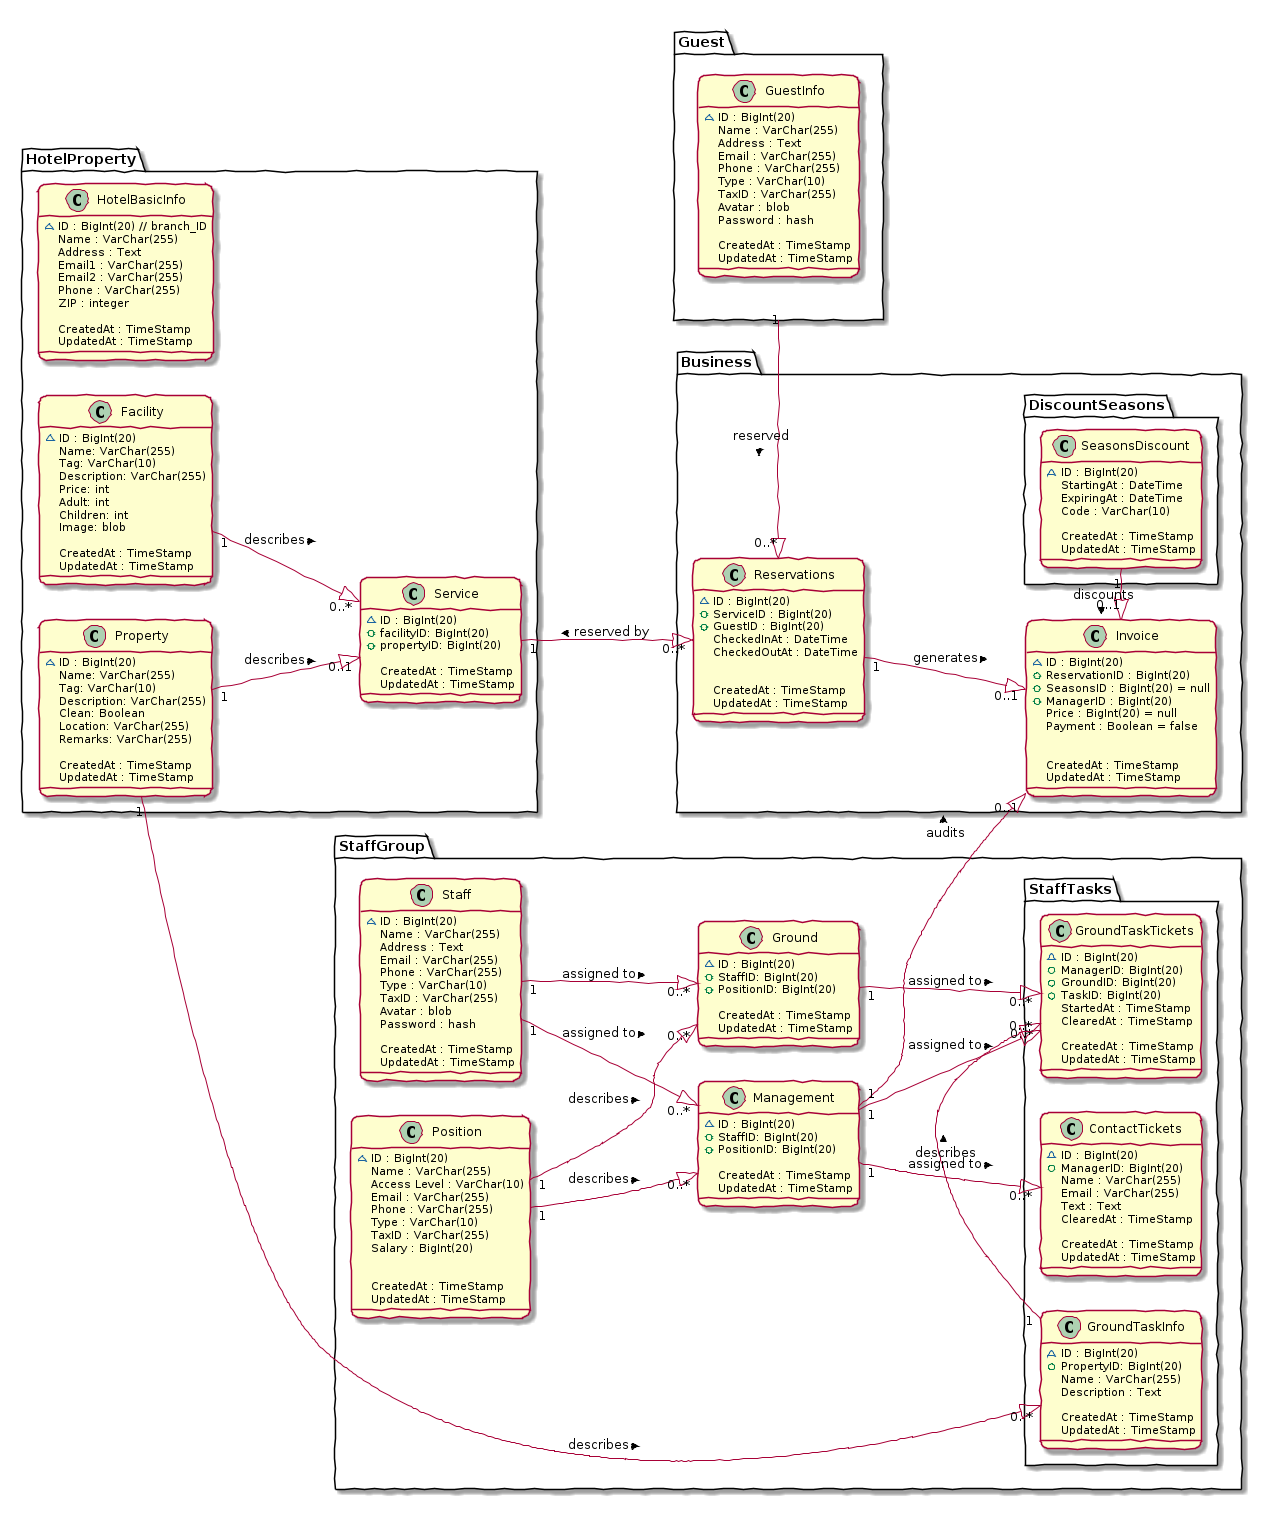
\includegraphics[width=16cm]{fig/HotelERD}}
	%{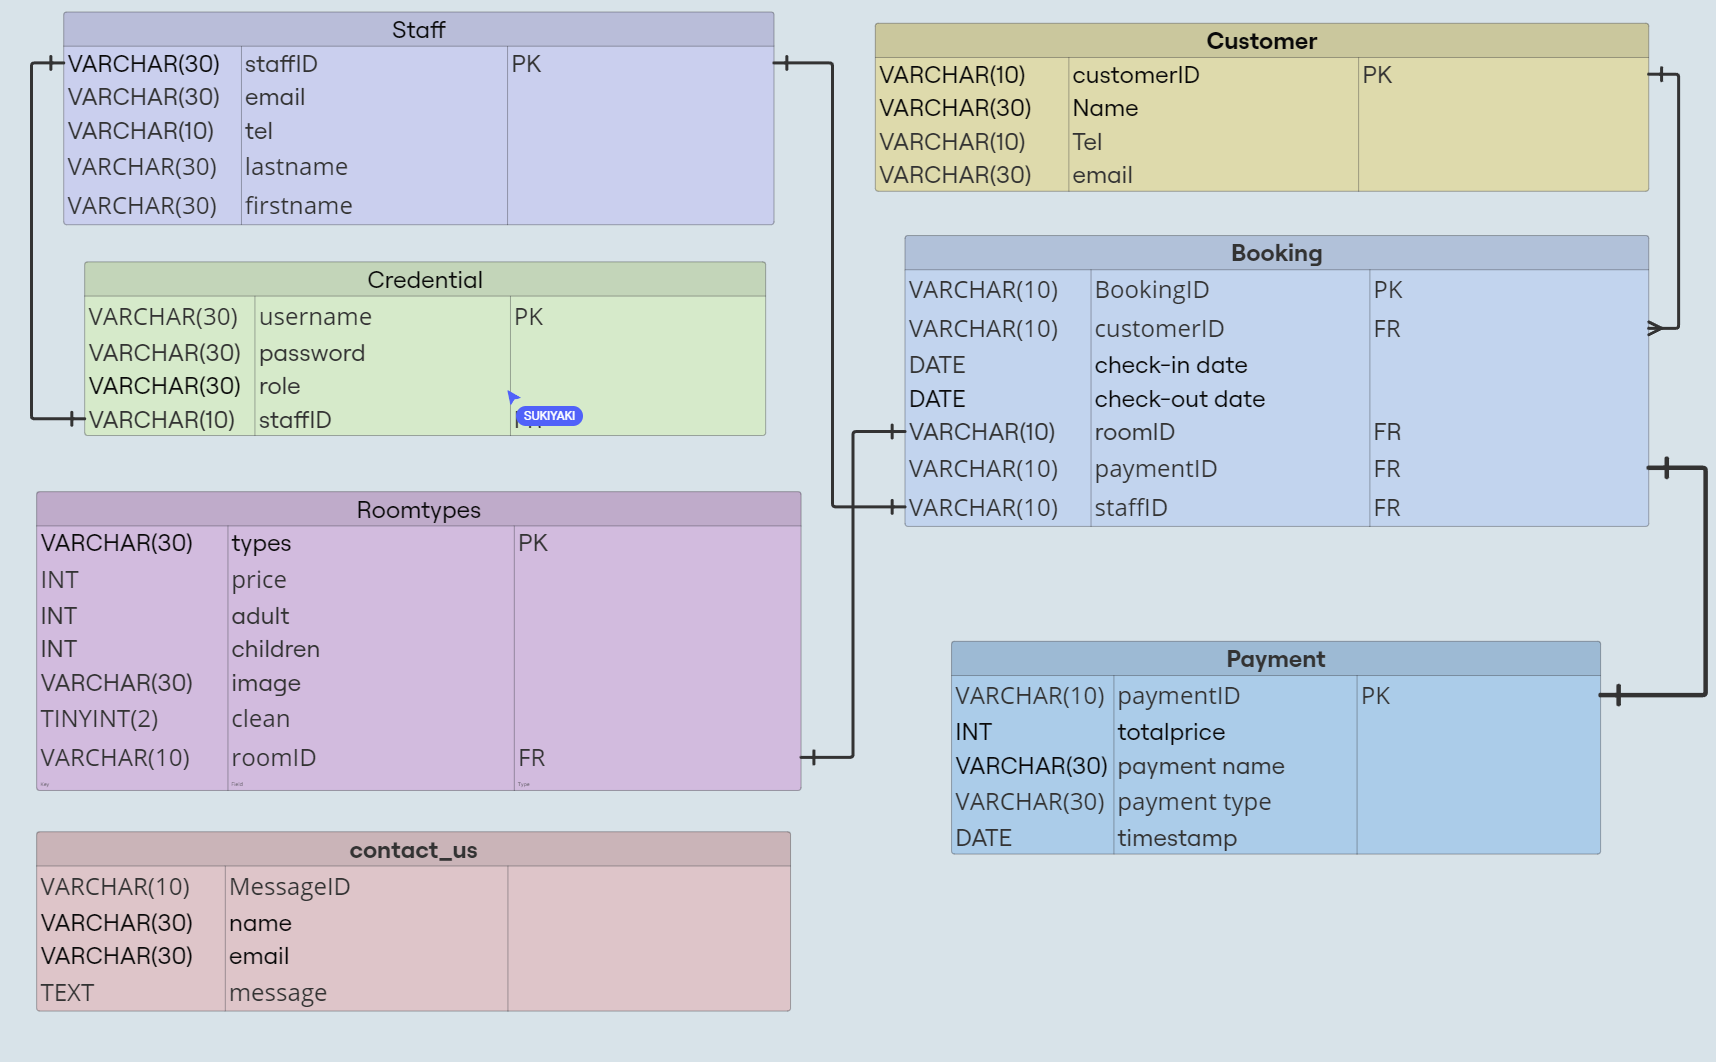
\includegraphics[]{fig/ERD_v1}}
	\caption{Final version for ER model diagram}
\end{figure} 

\section{Data Dictionary}

\begin{table}[H]
	\centering
	\begin{tabular}{cllll}
		\hline
		Field Name & Data type & Field size & Constraints & Description \\ \hline
		\texttt{ID} & \texttt{BIGINT} & 20 & \texttt{PK} & Auto-increment \\
		
		\texttt{CreatedAt} & \texttt{TIMESTAMP} & \texttt{AUTO} & \texttt{NOT NULL} & Auto \\
		\texttt{UpdatedAt} & \texttt{TIMESTAMP} & \texttt{AUTO} & \texttt{NOT NULL} & Auto \\
		\hline
	\end{tabular}
	\caption{Basic Format for Data Dictionary}
\end{table}

\subsection{Guest Information}

\begin{table}[H]
	\centering
	\begin{tabular}{cllll}
		\hline
		Field Name & Data type & Field size & Constraints & Description \\ \hline
		\texttt{ID} & \texttt{BIGINT} & 20 & \texttt{PK} & Auto-increment \\
		\texttt{Name} & \texttt{VARCHAR} & 255 & \texttt{NOT NULL} &  \\
		\texttt{Address} & \texttt{TEXT} & & \texttt{NOT NULL} &  \\
		\texttt{Email} & \texttt{VARCHAR} & 255 & \texttt{NOT NULL} &  \\
		\texttt{Phone} & \texttt{VARCHAR} & 255 & \texttt{NOT NULL} &  \\
		\texttt{Type} & \texttt{VARCHAR} & 10 & \texttt{NOT NULL} & Individual or Organization  \\
		\texttt{TaxID} & \texttt{VARCHAR} & 255 & &  \\
		\texttt{Avatar} & \texttt{BLOB} &  & &  \\
		\texttt{Password} & \texttt{HASH} &  & \texttt{NOT NULL} &  \\
		
		\texttt{CreatedAt} & \texttt{TIMESTAMP} & \texttt{AUTO} & \texttt{NOT NULL} & Auto \\
		\texttt{UpdatedAt} & \texttt{TIMESTAMP} & \texttt{AUTO} & \texttt{NOT NULL} & Auto \\
		\hline
	\end{tabular}
	\caption{Guest Info Table}
\end{table}

\subsection{Hotel Property}

\subsubsection{Hotel Basic Information}

\begin{table}[H]
	\centering
	\begin{tabular}{cllll}
		\hline
		Field Name & Data type & Field size & Constraints & Description \\ \hline
		\texttt{ID} & \texttt{BIGINT} & 20 & \texttt{PK} & Auto-increment \\
		\texttt{Name} & \texttt{VARCHAR} & 255 & \texttt{NOT NULL} &  \\
		\texttt{Address} & \texttt{TEXT} & & \texttt{NOT NULL} &  \\
		\texttt{Email1} & \texttt{VARCHAR} & 255 & \texttt{NOT NULL} &  \\
		\texttt{Email2} & \texttt{VARCHAR} & 255 & \texttt{NOT NULL} &  \\
		\texttt{Phone} & \texttt{VARCHAR} & 255 & \texttt{NOT NULL} &  \\
		\texttt{ZIP} & \texttt{INT} & 10 & &  \\
		
		\texttt{CreatedAt} & \texttt{TIMESTAMP} & \texttt{AUTO} & \texttt{NOT NULL} & Auto \\
		\texttt{UpdatedAt} & \texttt{TIMESTAMP} & \texttt{AUTO} & \texttt{NOT NULL} & Auto \\
		\hline
	\end{tabular}
	\caption{Hotel Basic Information Table}
\end{table}

\subsubsection{Facility: Hotel Service Offerings}

Now, this is the service offerings category. Another relation \texttt{Service} is associated which takes features of this relation and map them with individual rooms. Take this is type of Room (say Deluxe) that guests can book.

\begin{table}[H]
	\centering
	\begin{tabular}{cllll}
		\hline
		Field Name & Data type & Field size & Constraints & Description \\ \hline
		\texttt{ID} & \texttt{BIGINT} & 20 & \texttt{PK} & Auto-increment \\
		\texttt{Name} & \texttt{VARCHAR} & 255 & \texttt{NOT NULL} &  \\
		\texttt{Tag} & \texttt{VARCHAR} & 10 & \texttt{NOT NULL} &  \\
		\texttt{Description} & \texttt{VARCHAR} & 255 & \texttt{NOT NULL} &  \\
		\texttt{Price} & \texttt{INT} & & \texttt{NOT NULL} &  \\
		\texttt{Adult} & \texttt{INT} & & \texttt{NOT NULL} &  \\
		\texttt{Children} & \texttt{INT} & & \texttt{NOT NULL} &  \\
		\texttt{Image} & \texttt{BLOB} & & &  \\
		
		\texttt{CreatedAt} & \texttt{TIMESTAMP} & \texttt{AUTO} & \texttt{NOT NULL} & Auto \\
		\texttt{UpdatedAt} & \texttt{TIMESTAMP} & \texttt{AUTO} & \texttt{NOT NULL} & Auto \\
		\hline
	\end{tabular}
	\caption{Hotel Facilities Table}
\end{table}

\subsubsection{Property: Elements of Hotel Premises}

This can be rooms, hallway or any entity within the compound. Ground staff handle them. However, only few components in compound such as room and hallway can get Service status. We will see that in below subsection.

\begin{table}[H]
	\centering
	\begin{tabular}{cllll}
		\hline
		Field Name & Data type & Field size & Constraints & Description \\ \hline
		\texttt{ID} & \texttt{BIGINT} & 20 & \texttt{PK} & Auto-increment \\
		\texttt{Name} & \texttt{VARCHAR} & 255 & \texttt{NOT NULL} &  \\
		\texttt{Tag} & \texttt{VARCHAR} & 10 & \texttt{NOT NULL} &  type (room, banquet)\\
		\texttt{Description} & \texttt{VARCHAR} & 255 & \texttt{NOT NULL} &  \\
		\texttt{Clean} & \texttt{BOOLEAN} & & \texttt{NOT NULL} &  \\
		\texttt{Location} & \texttt{VARCHAR} & 255 & \texttt{NOT NULL} &  \\
		\texttt{Remarks} & \texttt{VARCHAR} & 255 & \texttt{NOT NULL} &  \\
		
		\texttt{CreatedAt} & \texttt{TIMESTAMP} & \texttt{AUTO} & \texttt{NOT NULL} & Auto \\
		\texttt{UpdatedAt} & \texttt{TIMESTAMP} & \texttt{AUTO} & \texttt{NOT NULL} & Auto \\
		\hline
	\end{tabular}
	\caption{Hotel Property Table}
\end{table}

\subsubsection{Service}

Now, this is the individual entity guests can use for reservation.

\begin{table}[H]
	\centering
	\begin{tabular}{cllll}
		\hline
		Field Name & Data type & Field size & Constraints & Description \\ \hline
		\texttt{ID} & \texttt{BIGINT} & 20 & \texttt{PK} & Auto-increment \\
		\texttt{facilityID} & \texttt{BIGINT} & 20 & \texttt{FK} &  \\
		\texttt{propertyID} & \texttt{BIGINT} & 20 & \texttt{FK} &  \\
		
		\texttt{CreatedAt} & \texttt{TIMESTAMP} & \texttt{AUTO} & \texttt{NOT NULL} & Auto \\
		\texttt{UpdatedAt} & \texttt{TIMESTAMP} & \texttt{AUTO} & \texttt{NOT NULL} & Auto \\
		\hline
	\end{tabular}
	\caption{Hotel Service Table}
\end{table}

\subsection{Business Context}

\subsubsection{Reservations}

\begin{table}[H]
	\centering
	\begin{tabular}{cllll}
		\hline
		Field Name & Data type & Field size & Constraints & Description \\ \hline
		\texttt{ID} & \texttt{BIGINT} & 20 & \texttt{PK} & Auto-increment \\
		\texttt{ServiceID} & \texttt{BIGINT} & 20 & \texttt{FK} &  \\
		\texttt{GuestID} & \texttt{BIGINT} & 20 & \texttt{FK} &  \\
		\texttt{CheckedInAt} & \texttt{DATETIME} & & &  \\
		\texttt{CheckedOutAt} & \texttt{DATETIME} & & &  \\
		
		\texttt{CreatedAt} & \texttt{TIMESTAMP} & \texttt{AUTO} & \texttt{NOT NULL} & Auto \\
		\texttt{UpdatedAt} & \texttt{TIMESTAMP} & \texttt{AUTO} & \texttt{NOT NULL} & Auto \\
		\hline
	\end{tabular}
	\caption{Reservations Table}
\end{table}

\subsubsection{Seasons Discount}

\begin{table}[H]
	\centering
	\begin{tabular}{cllll}
		\hline
		Field Name & Data type & Field size & Constraints & Description \\ \hline
		\texttt{ID} & \texttt{BIGINT} & 20 & \texttt{PK} & Auto-increment \\
		\texttt{StartingAt} & \texttt{DATETIME} & & &  \\
		\texttt{ExpiringAt} & \texttt{DATETIME} & & &  \\
		\texttt{Code} & \texttt{VARCHAR} & 10 & \texttt{NOT NULL} &  \\
		
		\texttt{CreatedAt} & \texttt{TIMESTAMP} & \texttt{AUTO} & \texttt{NOT NULL} & Auto \\
		\texttt{UpdatedAt} & \texttt{TIMESTAMP} & \texttt{AUTO} & \texttt{NOT NULL} & Auto \\
		\hline
	\end{tabular}
	\caption{Seasons Discount Table}
\end{table}

\subsubsection{Invoice}

\begin{table}[H]
	\centering
	\begin{tabular}{cllll}
		\hline
		Field Name & Data type & Field size & Constraints & Description \\ \hline
		\texttt{ID} & \texttt{BIGINT} & 20 & \texttt{PK} & Auto-increment \\
		\texttt{ReservationsID} & \texttt{BIGINT} & 20 & \texttt{FK} &  \\
		\texttt{SeasonsID} & \texttt{BIGINT} & 20 & \texttt{FK, NULL} & \\
		\texttt{ManagerID} & \texttt{BIGINT} & 20 & \texttt{FK} & \\
		\texttt{Price} & \texttt{BIGINT} & 20 & &  \\
		\texttt{Payment} & \texttt{BOOLEAN} & & \texttt{DEFAULT = FALSE} &  \\
		
		\texttt{CreatedAt} & \texttt{TIMESTAMP} & \texttt{AUTO} & \texttt{NOT NULL} & Auto \\
		\texttt{UpdatedAt} & \texttt{TIMESTAMP} & \texttt{AUTO} & \texttt{NOT NULL} & Auto \\
		\hline
	\end{tabular}
	\caption{Invoice Table}
\end{table}

\subsection{Staff Operations}

\subsubsection{Staff}

\begin{table}[H]
	\centering
	\begin{tabular}{cllll}
		\hline
		Field Name & Data type & Field size & Constraints & Description \\ \hline
		\texttt{ID} & \texttt{BIGINT} & 20 & \texttt{PK} & Auto-increment \\
		\texttt{Name} & \texttt{VARCHAR} & 255 & \texttt{NOT NULL} &  \\
		\texttt{Address} & \texttt{TEXT} & & \texttt{NOT NULL} &  \\
		\texttt{Email} & \texttt{VARCHAR} & 255 & \texttt{NOT NULL} &  \\
		\texttt{Phone} & \texttt{VARCHAR} & 255 & \texttt{NOT NULL} &  \\
		\texttt{Type} & \texttt{VARCHAR} & 10 & \texttt{NOT NULL} & Internship status  \\
		\texttt{TaxID} & \texttt{VARCHAR} & 255 & & Personal ID \\
		\texttt{Avatar} & \texttt{BLOB} &  & &  \\
		\texttt{Password} & \texttt{HASH} &  & \texttt{NOT NULL} &  \\
		
		\texttt{CreatedAt} & \texttt{TIMESTAMP} & \texttt{AUTO} & \texttt{NOT NULL} & Auto \\
		\texttt{UpdatedAt} & \texttt{TIMESTAMP} & \texttt{AUTO} & \texttt{NOT NULL} & Auto \\
		\hline
	\end{tabular}
	\caption{Staff Info Table}
\end{table}

\subsubsection{Position}

This is a metadata table for the list of positions in hotel.

\begin{table}[H]
	\centering
	\begin{tabular}{cllll}
		\hline
		Field Name & Data type & Field size & Constraints & Description \\ \hline
		\texttt{ID} & \texttt{BIGINT} & 20 & \texttt{PK} & Auto-increment \\
		\texttt{Name} & \texttt{VARCHAR} & 255 & \texttt{NOT NULL} &  \\
		\texttt{Access Level} & \texttt{VARCHAR} & 10 & \texttt{NOT NULL} &  \\
		\texttt{Email} & \texttt{VARCHAR} & 255 & \texttt{NOT NULL} &  \\
		\texttt{Phone} & \texttt{VARCHAR} & 255 & \texttt{NOT NULL} &  \\
		\texttt{Type} & \texttt{VARCHAR} & 10 & \texttt{NOT NULL} &  \\
		\texttt{TaxID} & \texttt{VARCHAR} & 255 & &  Tax Code\\
		\texttt{Salary} & \texttt{BIGINT} & 20 & &  \\
		
		\texttt{CreatedAt} & \texttt{TIMESTAMP} & \texttt{AUTO} & \texttt{NOT NULL} & Auto \\
		\texttt{UpdatedAt} & \texttt{TIMESTAMP} & \texttt{AUTO} & \texttt{NOT NULL} & Auto \\
		\hline
	\end{tabular}
	\caption{Position Info Table}
\end{table}

\subsubsection{Ground Staff}

\begin{table}[H]
	\centering
	\begin{tabular}{cllll}
		\hline
		Field Name & Data type & Field size & Constraints & Description \\ \hline
		\texttt{ID} & \texttt{BIGINT} & 20 & \texttt{PK} & Auto-increment \\
		\texttt{StaffID} & \texttt{BIGINT} & 20 & \texttt{FK} &  \\
		\texttt{PositionID} & \texttt{BIGINT} & 20 & \texttt{FK} &  \\
		
		\texttt{CreatedAt} & \texttt{TIMESTAMP} & \texttt{AUTO} & \texttt{NOT NULL} & Auto \\
		\texttt{UpdatedAt} & \texttt{TIMESTAMP} & \texttt{AUTO} & \texttt{NOT NULL} & Auto \\
		\hline
	\end{tabular}
	\caption{Ground Staff Info Table}
\end{table}

\subsubsection{Management Staff}

\begin{table}[H]
	\centering
	\begin{tabular}{cllll}
		\hline
		Field Name & Data type & Field size & Constraints & Description \\ \hline
		\texttt{ID} & \texttt{BIGINT} & 20 & \texttt{PK} & Auto-increment \\
		\texttt{StaffID} & \texttt{BIGINT} & 20 & \texttt{FK} &  \\
		\texttt{PositionID} & \texttt{BIGINT} & 20 & \texttt{FK} &  \\
		
		\texttt{CreatedAt} & \texttt{TIMESTAMP} & \texttt{AUTO} & \texttt{NOT NULL} & Auto \\
		\texttt{UpdatedAt} & \texttt{TIMESTAMP} & \texttt{AUTO} & \texttt{NOT NULL} & Auto \\
		\hline
	\end{tabular}
	\caption{Management Staff Info Table}
\end{table}

\subsubsection{Staff Tasks}

\begin{table}[H]
	\centering
	\begin{tabular}{cllll}
		\hline
		Field Name & Data type & Field size & Constraints & Description \\ \hline
		\texttt{ID} & \texttt{BIGINT} & 20 & \texttt{PK} & Auto-increment \\
		\texttt{ManagerID} & \texttt{BIGINT} & 20 & \texttt{FK} &  \\
		\texttt{GroundID} & \texttt{BIGINT} & 20 & \texttt{FK} &  \\
		\texttt{TaskID} & \texttt{BIGINT} & 20 & \texttt{FK} &  \\
		\texttt{StartedAt} & \texttt{TIMESTAMP} & & &  \\
		\texttt{ClearedAt} & \texttt{TIMESTAMP} & & &  \\

		\texttt{CreatedAt} & \texttt{TIMESTAMP} & \texttt{AUTO} & \texttt{NOT NULL} & Auto \\
		\texttt{UpdatedAt} & \texttt{TIMESTAMP} & \texttt{AUTO} & \texttt{NOT NULL} & Auto \\
		\hline
	\end{tabular}
	\caption{Ground Tasks Ticket Table}
\end{table}

\begin{table}[H]
	\centering
	\begin{tabular}{cllll}
		\hline
		Field Name & Data type & Field size & Constraints & Description \\ \hline
		\texttt{ID} & \texttt{BIGINT} & 20 & \texttt{PK} & Auto-increment \\
		\texttt{PropertyID} & \texttt{BIGINT} & 20 & \texttt{FK} &  \\
		\texttt{Name} & \texttt{VARCHAR} & 255 & \texttt{NOT NULL} &  \\
		\texttt{Description} & \texttt{TEXT} &  & \texttt{} &  \\

		\texttt{CreatedAt} & \texttt{TIMESTAMP} & \texttt{AUTO} & \texttt{NOT NULL} & Auto \\
		\texttt{UpdatedAt} & \texttt{TIMESTAMP} & \texttt{AUTO} & \texttt{NOT NULL} & Auto \\
		\hline
	\end{tabular}
	\caption{Ground Tasks Information Table}
\end{table}

This table is also a metadata table for assigning tasks.

\begin{table}[H]
	\centering
	\begin{tabular}{cllll}
		\hline
		Field Name & Data type & Field size & Constraints & Description \\ \hline
		\texttt{ID} & \texttt{BIGINT} & 20 & \texttt{PK} & Auto-increment \\
		\texttt{ManagerID} & \texttt{BIGINT} & 20 & \texttt{FK} &  \\
		\texttt{Name} & \texttt{VARCHAR} & 255 & \texttt{NOT NULL} &  \\
		\texttt{Email} & \texttt{VARCHAR} & 255 & \texttt{NOT NULL} &  \\
		\texttt{Text} & \texttt{TEXT} &  & \texttt{} &  \\
		\texttt{ClearedAt} & \texttt{TIMESTAMP} & & &  \\

		\texttt{CreatedAt} & \texttt{TIMESTAMP} & \texttt{AUTO} & \texttt{NOT NULL} & Auto \\
		\texttt{UpdatedAt} & \texttt{TIMESTAMP} & \texttt{AUTO} & \texttt{NOT NULL} & Auto \\
		\hline
	\end{tabular}
	\caption{Contact Tickets Table}
\end{table}

\clearpage
%=========================================================